% !Mode:: "TeX:UTF-8"
% !TEX program  = xelatex
\documentclass[a4paper]{article}
\usepackage{amsmath}
\usepackage{amssymb}
\usepackage{ctex}
\usepackage{braket}
%\usepackage[european]{circuitikz}
\usepackage{multirow}
\usepackage{float}
\usepackage{colortbl}
\usepackage{graphicx}
\usepackage{geometry}
\geometry{left=2.5cm,right=2.5cm,bottom=2.5cm,top=2.5cm}

\usepackage{physics}
\usepackage{mhchem}
\usepackage{siunitx}
\usepackage{bm}
\DeclareMathOperator{\e}{\mathrm{e}}
\DeclareMathOperator{\I}{\mathrm{i}}


\title{近代物理实验报告:单电子固态量子计算}
\author{\quad 学号\quad 匡亚明学院}
\date{2019年2月29日}
\begin{document}
\maketitle
\bibliographystyle{unsrt}

\tableofcontents
\newpage
%--------main-body------------

\section{引言}


%\section{实验目的}
\subsection{量子计算背景}
过去的几十年中,经典计算机经历了快速的发展时期。第一台通用电子计算机ENIAC
占地约170平方米,如今的掌上电脑已经可以放进口袋。体积的巨大变化,主要归功
于集成电路工业的飞速发展。英特尔公司创始人之一戈登·摩尔曾提出著名的摩尔定
律,用以总结和预期集成电路的发展,即集成电路上可容纳的晶体管数目,约每隔18
个月便会翻一倍,其性能也会翻倍。然而随着电路集成度越来越高,摩尔定律也遇到
了新的挑战。因为按照摩尔定律描述的发展趋势,集成电路的工艺己进入纳米尺度。
在芯片上如此高密度的集成元器件,热耗散问题是一个巨大的挑战。更严重的是,随
着集成电路的工艺进入纳米尺度,量子效应会逐渐显现并占据支配地位。当描述元器
件工作的物理规律由经典物理转变为量子力学,试图按照原来的方式保持集成电路的
发展趋势就非常困难了。

既然在微观尺度下,量子力学效应占主导,那有没有可能利用量子力学效应来构
造计算机呢?费曼最先在1982年指出,采用经典计算机不可能以有效方式来模拟量子
系统的演化。我们知道,经典计算机与量子系统遵从不同的物理规律,用于描述量子
态演化所需要的经典信息量,远远大于用来以同样精度描述相应的经典系统所需的经
典信息量。费曼提出用量子计算则可以精确而方便地实现这种模拟。1985 年,David
Deutsch深入研究了量子计算机是否比经典计算机更有效率的问题。他首次在理论上
描述出了量子计算机的简单模型——量子图灵机模型,研究了它的一般性质,预言了
它的潜在能力。但当时的人们还不知道有什么具体的可求解问题,量子计算能比经典
计算更有优越性。1994年,美国数学家Peter Shor从原理上指出,量子计算机可以用
比经典计算机快得多的速度来求解大数的质因子分解问题。由于大数质因子分解问题
是现代通信与信息安全的基石,Shor的开创性工作引起了巨大的关注,其可期待的辉
煌应用潜力有力地刺激了量子计算机和量子密码等领域的研究发展,成为量子信息科
学发展的重要里程碑之一。1996 年Grover发现了另一种很有用的量子算法,即所谓
的量子搜索算法,它适用于解决如下问题: 从$ N $个未分类的客体中寻找出某个特定的
客体。经典算法只能是一个接一个地搜寻,直到找到所要的客体为止,这种算法平均
地讲要寻找$ N/2 $次,成功几率为$ 1/2 $,而采用Grover的量子算法则只需要
$ \sqrt{N} $次。

随着一系列量子算法的提出,量子计算对某些重要问题相对于己知的经典计算方
式的计算能力的展现出巨大的优势。量子计算不仅吸引着众多的科研人员,其应用前
景也吸引了谷歌、微软、IBM 等国际知名公司参与这一领域的竞争。近年来,各研究团队更是试图实现“量子霸权”(Quantum supremacy),即通过量子计算实现对经典计算能力的极限的突破

\section{实验原理}
\subsection{量子计算基本概念}
经典计算机需要信息的载体,逻辑操作,状态读出等一系列基本元素。量子计算机也
类似,首先我们需要量子信息的载体,即量子比特。然后需要具备对量子比特进行初
始化,操控和读出的能力。我们利用一系列的逻辑操作,构成量子算法,来实现特定
的计算目的。
\subsubsection{量子比特}
\begin{figure}[H]
	\centering
	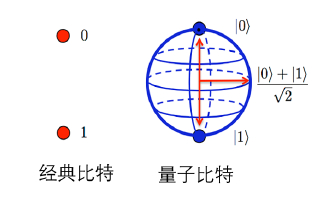
\includegraphics[width=0.4\linewidth]{fig/1.jpg}
	\caption{经典比特与量子比特对比示意图}
\end{figure}
如果我们把数据送入计算机处理,就必须把数据表示成为计算机能识别的形式。
在经典计算机中,信息单元用1个二进制位表示,它处于“0”态或“1”态。而在量子
计算机中,信息单元称为“量子比特”,它除了可以处于“0”态或“1”态外,还可处
于一种叠加态。我们用$ \ket{0} $和$ \ket{1} $表示量子比特可取的状态基失,单个量子比特可取的为
\begin{equation}\label{key}
\ket{Psi} = \alpha\ket{0} + \beta\ket{1}
\end{equation}
由于$ \alpha^*\alpha + \beta^*\beta = 1 $,们也可以这样表示量子比特:
\begin{equation}\label{key}
\ket{\Psi} = \cos\dfrac{\theta}{2}\ket{0} + \e^{\I\phi}\sin\dfrac{\theta}{2}\ket{1}
\end{equation}
其中$ -\pi \leq \theta \leq \pi, 0\leq \phi \leq 2\pi $. 显然$ \theta $和
$ \phi $在单位三维球体上定义了一个点,这个球体通常被称为布洛赫球。单个量子比特的
纯态可以与布洛赫球面上的点一一对应.

\subsubsection{量子逻辑门}
经典计算中用到很多基本逻辑门,包括与门、或门、非门、异或门、与非门和或非门
等,这些元件组合在一起能构成用来计算任何函数的硬件电路。量子计算机与此类
似,也由一系列的量子门组合而成,以此来完成复杂计算任务。图(\ref{fig:gate})列出了常用的量子逻辑门,其代表符号和矩阵表示。描述单个量子门的矩阵$ U $要求必须是幺正的,
即$ U U^\dagger = I $. C-NOT门是一个两比特门,当控制比特是$ \ket{0} $时,目标比特不变。当控制比特是$ \ket{1} $时,目标比特发生翻转。\\
\begin{figure}[H]
	\centering
	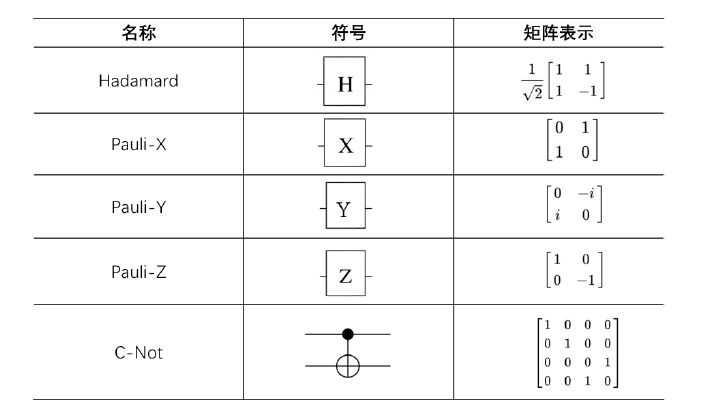
\includegraphics[width=0.8\linewidth]{fig/2.jpg}
	\caption{常用量子逻辑门的符号和矩阵表示}
	\label{fig:gate}
\end{figure}
要实现实用的量子计算,需要的量子比特的数目远不止两个,因此需要能够实现多比特的量子逻辑门。而且,量子计算中需要施加的量子逻辑门与要解决的问题有关,也就是说,为了解决不同的问题,需要使用不同的量子逻辑门。那么,能不能只用一些基本的量子逻辑门,来实现任意的量子逻辑门的效果呢? 理论上可以证明,对于任意的多比特量子逻辑门,都可以通过两比特受控非门结合单比特量子逻辑门的方式实现。我们称单比特量子逻辑门和受控非门形成一组普适的量子逻辑门。

\subsubsection{量子测量}
为了得到量子计算的结果,需要对末态进行量子测量。对于量子比特$ \ket{\Psi} = \alpha\ket{0} + \beta\ket{1} $,采用基矢$ \ket{0} $,$ \ket{1} $进行测量,得到结果$ \ket{0} $和$ \ket{1} $的几率分别为$ \abs{\alpha}^2 $和$ \abs{\beta}^2 $。如
果选择另外的一组正交基矢:
\begin{equation}\label{key}
\ket{+} = \dfrac{1}{\sqrt{2}}(\ket{0} + \ket{1})  \qquad \ket{-} = \dfrac{1}{\sqrt{2}}(\ket{0} - \ket{1})
\end{equation}
任意量子比特的态可以写成:
\begin{equation}\label{key}
\ket{\Psi} = \alpha\ket{0} + \beta\ket{1} = \dfrac{\alpha+\beta}{\sqrt{2}}\ket{+} + \dfrac{\alpha-\beta}{\sqrt{2}}\ket{-}
\end{equation}
测量之后,坍缩到$ \ket{+} $或者$ \ket{-} $的几率分别为$ \abs{\alpha+\beta}^2/2 $,$ \abs{\alpha-\beta}^2/2 $.\\
一般情况下,给出任意的基矢$ \ket{a} $和$ \ket{b} $,可以将任意态表示为$ \alpha\ket{a}+ \beta\ket{b} $,只要$ \ket{a} $和$ \ket{b} $是正交的,就可以进行相对于$ \ket{a} $和$ \ket{b} $的测量,以$ \abs{\alpha}^2 $的几率得到$ \ket{a} $,以$ \abs{\beta}^2 $的几率得到$ \ket{b} $。
\subsubsection{量子算法}
经典计算机在处理某些问题的时候,速度是很快的,比如计算乘法$ 127\cross 229 = \text{?} $。但如果将这个问题反过来,求解29083这个数能分解成哪两个质数是乘积$ \text{?}\cross\text{?} = 29083 $,这时候经典计算机可能要花费很长的时间来处理。尤其是当要分解的数非常大的时候,普通计算可能要运算几年或者更长的时间才能得到结果。而此时如果采用量子算法,则大数质因子分解问题可以迎刃而解。利用量子计算机,几乎可以瞬间完成大数分解。\\
量子算法与经典算法相比,其差别在于,量子算法融入了量子力学的很多特征。
经典算法本质上不依赖于量子物理,只是数学上的技巧。而量子算法中用到了量子相
干性、量子叠加性、量子并行性、波函数坍缩等量子力学特性,进而大大提高了来计
算效率。这种崭新的计算模式,给计算科学带来重大影响。有些问题,依据经典计算
复杂性理论,是不存在有效算法的,但在量子算法的框架里却找到了有效法。最为典
型的量子算法有:Shor算法(质因数分解),QEA算法(组合优化求解),Grover算法
(量子搜索算法)等。这些量子算法可能处理的问题不同,但是都是采用了量子力学
物理性质进行计算。每一种算法都有其独特性,比如Shor算法对质因素分解将直接
威胁RSA加密体系,Grover算法在搜索方面,指数级的加速。这些都有潜在的应用价
值。下面我们以Deutsch-Jozsa算法为例,说明量子并行性的优势。\\
\paragraph{Deutsch-Jozsa算法}~\\
考虑定义在$ \{0,1\}^n $上的函数$ f(x) $,满足$ f(x)\in \{0, 1\} $,且$ f(x) $的输出分为两种情况。
一种是,对于任意输入,它只输出$ 0 $或者$ 1$,我们称之为常函数;另一种情况是,恰好对于一半的输入,输出为$ 0 $,另一半输入,输出为$ 1 $,我们称之为平衡函数。问题是:对于未知的$ f(x) $,我们要区分它是常函数还是平衡函数。如果采用经典计算的方式,需要挨个检查输出结果,要得到准确无误的判断,最坏的情况需要进行$ 2^{n-1} + 1  $次计算。这是因为,如果进行了$ 2^{n-1} $次计算后,得到的是$ 2^{n-1} $个相同的输出,这时候仍不能确定$ f(x)  $是常函数还是平衡函数。若果采用量子计算的方式,对于同样的问题,只需要一次计算就可以得出结果,解决这个问题的量子算法称为Deutsch-Jozsa算法(简称D-J算法)。D-J算法是1992年由David Deutsch和Richard Jozsa提出的,是对1985年David Deutsch单独提出的Deustsh算法的一般性推广。Deutsch算法即是D-J算法$ n=1  $的情况。因为Deutsch算法更易说明,下面我们就详细讲解Deutsch算法。\\
函数$ f(x) $,其定义域为$ \{0,1\} $,且$ f(x)\in\{0,1\} $,那么这样的函数共有四种情况,如下图所示:
\begin{figure}[H]
	\centering
	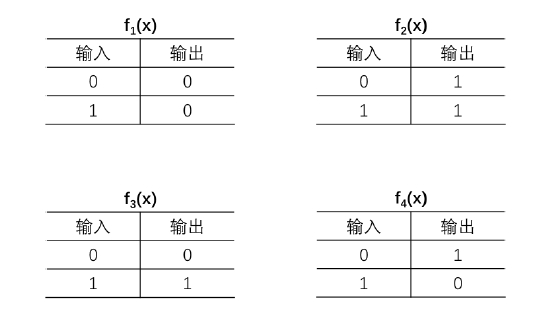
\includegraphics[width=0.65\linewidth]{fig/deutsch.jpg}
	\caption{常函数与平衡函数举例:$ f_1(x) $ 与$ f_2(x)  $是常函数,$ f_3(x) $与$ f_4(x) $是平衡函数。}
	\label{fig:deutsch}
\end{figure}
现在我们需要判断$ f(x)  $是常函数还是平衡函数,采用经典计算的方法,需要分
别计算$ f(0)  $和$ f(1) $,然后判断$ f(0)  $和$ f(1)  $是否相等,共需进行两次计算。如果采用量子计算中的Deutsch算法,则只需一次计算就能够判定。如图 (\ref{fig:deutsch2}) 所示,是Deutsch算法的量子线路图。该量子算法需要两个量子比特,其初态是$ \ket{a} = \ket{01} $,然后对两个比特分别施加Hadamard门,得到的态为:
\begin{equation}\label{key}
\ket{b} = \qty(\dfrac{\ket{0} + \ket{1}}{\sqrt{2}}) \qty(\dfrac{\ket{0} - \ket{1}}{\sqrt{2}})
\end{equation}
\begin{figure}[H]
	\centering
	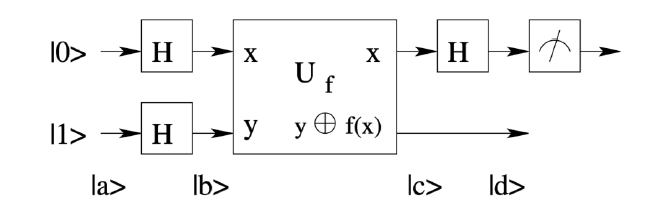
\includegraphics[width=0.8\linewidth]{fig/deutsch2.jpg}
	\caption{Deutsch算法的量子线路图}
	\label{fig:deutsch2}
\end{figure}
对$ \ket{b} $施加量子逻辑门$ U_f $,其中$ U_f $对量子比特态的作用为
\begin{equation}\label{key}
U_f\ket{x,y} = \ket{x,y\oplus f(x)}
\end{equation}
$ y\oplus f(x) $代表$ y+f(x) $以$ 2  $的余数。因此有
\begin{equation}\label{key}
\left\{\mqty{
	U_f\ket{x,0} &= \ket{x, f(x)}\\
	U_f\ket{x,1} &= \ket{x, 1-f(x)}
}\right.	
\end{equation}
所以
\begin{equation}\label{key}
U_f\ket{x} \qty(\dfrac{\ket{0} - \ket{1}}{\sqrt{2}}) = \ket{x} \qty(\dfrac{\ket{f(x)} - \ket{1-f(x)}}{\sqrt{2}}) = (-1)^{f(x)} \ket{x} \qty(\dfrac{\ket{0} - \ket{1}}{\sqrt{2}})
\end{equation}
如果$ f(0) =f(1) $,即$ f(x)  $是常函数,经过$ U_f $作用之后得到的态是:
\begin{equation}\label{key}
\ket{c} = \pm \qty(\dfrac{\ket{0} + \ket{1}}{\sqrt{2}})\qty(\dfrac{\ket{0} - \ket{1}}{\sqrt{2}})
\end{equation}
如果$ f(0) \neq f(1) $,即$ f(x)  $是平衡函数,经过$ U_f $作用之后得到的态是:
\begin{equation}\label{key}
\ket{c} = \pm \qty(\dfrac{\ket{0} - \ket{1}}{\sqrt{2}})\qty(\dfrac{\ket{0} - \ket{1}}{\sqrt{2}})
\end{equation}
算法运行到这一步,第一个量子比特的态,已经与$ f(x)  $是常函数还是平衡函数产生关
联。若$ f(x) $是常函数,则第一个量子比特的态是$ \qty(\dfrac{\ket{0} + \ket{1}}{\sqrt{2}}) $。若$ f(x)  $是平衡函数,则第一个
量子比特的态是$ \qty(\dfrac{\ket{0} - \ket{1}}{\sqrt{2}}) $。\\
然后对第一个量子比特施加Hadamard门,如果$ f(0) = f(1) $,
即$ f(x)  $是常函数,我们得到:
\begin{equation}\label{key}
\ket{d} = \pm\ket{0}\qty(\dfrac{\ket{0} - \ket{1}}{\sqrt{2}})
\end{equation}
如果$ f(0) \neq f(1) $,即$ f(x)  $是平衡函数,我们得到:
\begin{equation}\label{key}
\ket{d} = \pm\ket{1}\qty(\dfrac{\ket{0} - \ket{1}}{\sqrt{2}})
\end{equation}
以$ \ket{0} $和$ \ket{1} $作为基矢,对第一个量子比特进行测量。如果$ f(x)  $是常函数,则测量结果是$ 0 $;如果$ f(x)  $是平衡函数,则测量结果是$ 1 $。\\
总结一下Deutsch算法的过程,我们将量子比特制备到$ \ket{0} $和$ \ket{1} $的叠加态,只需进行一次计算,就可以根据末态的测量结果是$ 0  $还是$ 1 $,来判断$ f(x)  $是常函数还是平衡函数。根据经典算法,则需进行两次计算。将Deutsch算法的定义域从$ \{0,1\} $推广到$ \{0,1\}^n $,其解决方法即是D-J算法。D-J算法是最早提出的量子算法之一,虽然D-J算法解决的问题不具备太多实际意义,但该算法向人们展示了,解决某些问题时,量子计算能够比经典计算更高效。下面我们将讨论如何在实验上实现这一算法。

\subsection{量子计算的实验实现}
建造量子计算机的困难在于要找到一个可以编码量子比特,并且能够有效地被外
界控制,但又与环境有很好的隔离,不致使系统很快退相干失去量子特性的物理系
统。在介绍量子计算的物理实现技术之前,下面先介绍一下DiVincenzo关于量子计算
物理实现技术的判据。
\subsubsection{DiVincenzo判据}
2000年,DiVincenzo讨论了实现量子计算的物理要求,并提出了如下的7条判据:
\begin{enumerate}
	\item 可扩展的具有良好特性的量子比特系统;
	\item 能够制备量子比特到某个基准态;
	\item 具有足够长的相干时间来完成量子逻辑门操作;
    \item 能够实现一套通用量子逻辑门操作;
	\item 能够测量量子比特;
	\item 能够使飞行量子比特和静止量子比特互相转化;
	\item 能够使飞行量子比特准确地在不同的地方之间传送。
\end{enumerate}
后面两条是针对量子计算机之间通信提出的要求,前面五条是实现量子计算的要求。
人们已经在多种系统上试验了量子计算机的实现方案,包括离子阱、超导约瑟夫森
结、腔量子电动力学、硅基半导体、量子点、液体核磁共振等等。下面我们以金刚石
中的NV色心为例,说明量子计算的实验实现。

\subsubsection{金刚石中的NV色心}

NV(Nitrogen-Vacancy)色心是金刚石中的一种点缺陷。金刚石晶格中一个碳原子缺
失形成空位,近邻的位置有一个氮原子,这样就形成以了一个NV色心。我们这里所
说的NV色心,指的是带负电荷NV$ ^- $顺磁中心。NV色心的有六个电子,两个来自氮
原子,三个来自与空位相邻的碳原子,另外一个是俘获的(来自施主杂质的)电子。
\begin{figure}[H]
	\centering
	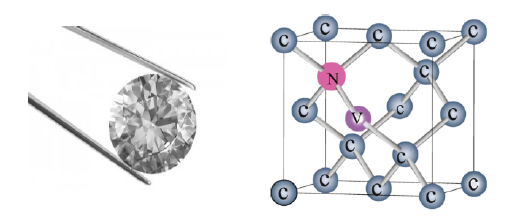
\includegraphics[width=0.8\linewidth]{fig/NV.jpg}
	\caption{金刚石和金刚石中的NV色心原子结构}
	\label{fig:NV}
\end{figure}

\subsubsection{自旋态初始化和读出}
\begin{figure}[H]
	\centering
	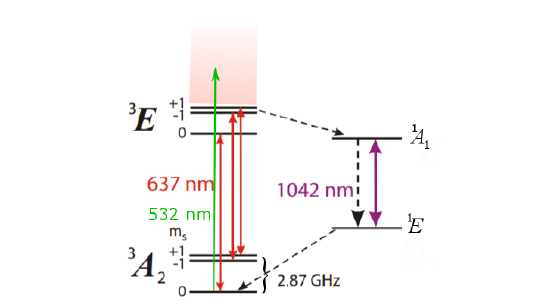
\includegraphics[width=0.8\linewidth]{fig/energy.jpg}
	\caption{室温下金刚石NV 色心的能级结构示意图。会辐射出光子的跃迁用实线箭头表
		示,非辐射跃迁用虚线箭头表示。}
	\label{fig:energy}
\end{figure}
图(\ref{fig:energy})是室温下金刚石NV色心的能级结构。NV色心的基态为自旋三重态,三重
态基态与激发态间跃迁相应的零声子线为$ \SI{637}{nm} $,红色区域为声子边带。基态的自旋三重态$ (\ket{m_s=0}, \ket{m_s=1}, \ket{m_s=-1}) $中,$ \ket{m_s=\pm 1} $在无磁场时是简并的,它们与$ \ket{m_s=0} $态之间的能隙(零场劈裂)对应微波频率为$ \SI{2.87}{GHz} $。激发态的能级自旋分裂对应的微波频率为$ \SI{1.4}{GHz} $。\\
首先$ \SI{532}{nm}  $的激光激发基态电子,由于电子跃迁是电偶极跃迁与电子自旋无
关,所以跃迁前后的自旋是守恒的。$ \ket{m_s=0} $的基态电子到$ \ket{m_s=0} $的声子边带,而$ \ket{m_s=\pm 1} $的基态电子到$ \ket{m_s=\pm 1} $的声子边带。之后$ \ket{m_s=0} $ 的电子绝大多数都直接跃迁到基态辐射荧光,而$ \ket{m_s=\pm 1} $的电子则一部分直接跃迁到基态辐射荧光,另一部分通过无辐射跃迁到单重态再到三重态的$ \ket{m_s=0} $态。经过多个周期之后,基态$ \ket{m_s=\pm 1} $上的布居度会越来越少,而$ \ket{m_s=0} $上的布居度会越来越多。这相
当于,在激光的照射下,布居度从$ \ket{m_s=\pm 1} $转移到了$ \ket{m_s=0} $,从而实现了自旋极化。常温下NV色心电子自旋的极化率可达$ 95\% $以上。\\
如果我们选取基态的$ \ket{m_s=0} $和$ \ket{m_s=1} $作为量子比特,NV色心的自旋极化就
对应于将量子比特的初态极化到$ \ket{0} $态。\\
由于$ \ket{m_s=\pm 1} $态有更大的概率通过无辐射跃迁,回到基态。所以$ \ket{m_s=0} $态的荧光比$ \ket{m_s=\pm 1} $态的荧光强度大,实验上得出大约大$ 20-40\% $。根据$ \ket{m_s=0} $态和$ \ket{m_s=\pm 1} $对应荧光强度的差别,就可以区分NV色心的自旋态,即实现对自旋量子比特状态的读出。由于由于单次实验得到的$ \ket{m_s=0} $态和$ \ket{m_s=\pm 1} $的荧光强度并不明显,室温下对NV色心电子自旋量子比特的测量一般为多次实验重复测量,测得的结果为某个观测量(如$ \ket{m_s=0}\bra{m_s=0} $) 的平均值。

\subsubsection{自旋态操控}
为了实现量子逻辑门,需要对NV色心的自旋状态进行操控。调控NV色心自旋态使用的是自旋磁共振技术,即利用微波场与自旋的相互作用,来调控自旋态的演化。
\begin{figure}[H]
	\centering
	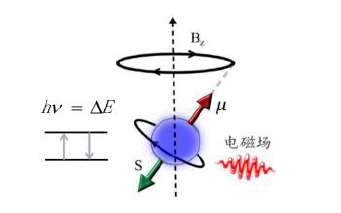
\includegraphics[width=0.5\linewidth]{fig/spin.jpg}
	\caption{自旋磁共振原理示意图}
	\label{fig:spin}
\end{figure}

\paragraph{磁场中自旋的薛定谔方程描述}~\\
量子力学中,描述量子态随时间演化的方程是薛定谔方程:
\begin{equation}\label{Schr}
H\Psi = \I\hbar\pdv{\Psi}{t}
\end{equation}
为了得到薛定谔方程的解,我们需要知道哈密顿量和初态波函数。考虑一个自旋$ 1/2 $
的电子,处在均匀外磁场中,系统哈密顿量可以表示为:
\begin{equation}
H = -\bm\mu\cdot\vb{B}_0     \label{H}
\end{equation}
其中,$ \bm\mu $是电子磁矩,$ \vb{B}_0 $是平行于$ z  $轴的静磁场。电子磁矩与自旋之间的关系是:
\begin{equation}\label{key}
\bm\mu = \gamma\vb{S}
\end{equation}
比例常数$ \gamma $被称作旋磁比。自旋算符$ \vb{S} = \tfrac{\hbar}{2}\bm\sigma $,其中$ \bm\sigma =  (\sigma_x, \sigma_y, \sigma_z)  $是泡利算符,其矩阵形式如下:
\begin{align}
\sigma_x = \mqty(0 & 1\\ 1 & 0) && 
\sigma_y = \mqty(0 & -\I\\ \I & 0) &&
\sigma_z = \mqty(1 & 0\\ 0 & -1)
\end{align}
代入$ \eqref{H} $可得
\begin{equation}
\label{HH}
H = -\dfrac{\hbar}{2}\mqty(\gamma B_0 & 0\\ 0 -\gamma B_0) 
= -\dfrac{\hbar}{2}\mqty(\omega_0 & 0\\ 0 -\omega_0) 
\end{equation}
该哈密顿量的本征能级是$ -\tfrac{1}{2}\hbar\omega_0 $和$ \tfrac{1}{2}\hbar\omega_0 $,分别对应自旋向上和向下的本征态。能级
差为$ \hbar\omega_0 $,恰好是频率为$ \omega_0 $的光子的能量。

\paragraph{自旋进动}
为了得到电子自旋在静磁场中的演化方程,我们记其自旋初态为
\begin{equation}\label{key}
\Psi_0(t) = a_0\ket{0} + b_0\ket{1}
\end{equation}
随时间演化的状态
\begin{equation}\label{key}
\Psi(t) = a\ket{0} + b\ket{1}
\end{equation}
其中
\begin{align}\label{key}
\ket{0} = \mqty(1\\ 0) & \qquad \ket{1} = \mqty(0\\ 1)
\end{align}
将$ \eqref{HH} $的哈密顿量带入薛定谔方程$ \eqref{Schr} $可以得到:
\begin{equation}\label{key}
\I\hbar\mqty(a\\ b) = -\dfrac{\hbar}{2}\mqty(\omega_0 & 0\\ 0 -\omega_0) \mqty(a\\ b)
\end{equation}
该方程的解是:
\begin{align}\label{key}
a = a_0\e^{\I \omega_0 t/2} &\quad  b = b_0\e^{\I \omega_0 t/2}
\end{align}
如果记$ \abs{a_0} = \cos(\alpha/2), \abs{b_0} = \sin(\alpha/2) $,那么可以得到:

\paragraph{共振微波驱动}

\section{实验装置}
实验所用仪器“金刚石量子计算教学机”,是以光探测磁共振为基本原理,以金刚石
NV色心为量子比特的量子计算教学设备。实验装置如图(\ref{fig:equip})所示。实验装置分为光学
模块、微波模块和控制脉冲发生模块,整机由运行在电脑上的软件控制。
%下面分别介绍各个模块的功能。
\begin{figure}[H]
	\centering
	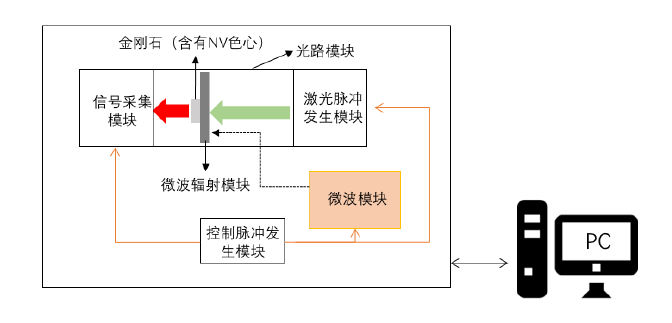
\includegraphics[width=0.9\linewidth]{fig/equip.jpg}
	\caption{实验装置图}
	\label{fig:equip}
\end{figure}

\section{实验内容及结果}
\subsection{启动}
\begin{enumerate}
	\item (1) 打开“金刚石量子计算教学机”背部的电源总开关,和前面板的银色金属开
	关,电源指示灯亮起,表示仪器正常上电;
	\item  打开电脑上控制软件Diamond I Studio,进入软件主界面。如图3.1所示;
	\item  点击“连接设备”按钮后,若显示“仪器已连接,请开始实验”,表示仪器已
	经可以进行实验。如果显示“仪器连接失败,请重新连接”。请再次点击“连接设备”
	按钮,直至仪器连接成功;
	
\end{enumerate}

\subsection{连续波实验}
\subsection{拉比振荡实验}
\subsection{$ T_2 $实验}
\subsection{D-J算法实验}
\subsection{设计实验}




%\section{实验数据}


\section{思考题}
\subsection*{请利用布洛赫球表示以下量子态:}

\subsection*{如果实验中施加的微波频率$ f $与共振频率$ f_0 $有偏差,即$ f = f_0 + \delta f $,拉比振荡的频率会如何变化?}

\subsection*{拉比振荡频率与微波功率的关系是什么?}

\subsection*{参照$ n=1 $的特殊情况,即图1.5所示的量子线路图,画出一般情况的D-J算法量子线路图,并解释算法原理}


%\nocite{jiaocai}
\bibliography{ref}
\end{document}